\chapter{Polly}
One of the numerous subprojects of the \llvm is Polly\footnote{The name \enquote{Polly} is a combination of \enquote{Polyhedral} and \enquote{\llvm}. \cite{PollyGrosser}} which provides plenty of options for automatic optimizations based on the polyhedral model operating on \llvmir.

\section{History}
Polly is an implementation of a loop optimizer based on the polyhedral model.\\
Before Polly there already existed an earlier implementation accessible using gcc.
The component for gcc was called Graphite and included the \pcp which is an independant interface between the \ir of gcc called GIMPLE\footnote{\draftnote{The name \enquote{GIMPLE} is a result of \enquote{gcc} and \enquote{Simple II}, on which GIMPLE is based. \cite{GenericGimple}}} and the internal \ir \gpoly.
The problem with it was, that GIMPLE is not made for being human readable.
As consequence to ease developing and to avoid plenty of bugs the implementation was transfered to be used with \llvm, whose \ir is more human readable.
Another advantage arises due to the fact, that \llvm is not bound to C or C++.
Currently Polly has to be loaded serving as a \llvm plugin.
In future releases Polly is going to be integrated directly into \llvm instead.

\section{The pipeline of Polly}
Polly is embeded in pipeline of \llvm.
More precisly it is called by the \opt (\autoref{subsec:optimizer}).
But before being able to use Polly the \llvmir has to be canonicalized.
The canonicalization is done by compiling the source code using clang with the options \texttt{-O3} and \texttt{-polly-canonicalize}.
Afterwards the library of Polly and its additional options can be loaded by the \opt.
\begin{figure}[!ht]
    \caption[The pipeline of Polly]{The pipeline of Polly \cite{PollyPresentation}.
    The figure shows the part of the pipeline of \llvm where Polly comes into effect.
    \tikzlegend}
    \centering
    \begin{tikzpicture}
        \coordinate(clang);
        \node(opt)[llvmIrNode, right=of clang]{\ac{LLVM} Optimizer};
        \node(polly)[llvmIrNode, below=of opt]{\ac{LLVM} Polly};
        \coordinate[right=of opt](generator);
        \path[llvmIrPath] (clang) to (opt);
        \path[llvmIrPath, bend right] (opt.south west) to node[auto, swap]{SCoP Detection} (polly);
        \path[llvmIrPath, bend right] (polly) to node[auto, swap]{Code Generation} (opt.south east);
        \path[llvmIrPath] (opt) to (generator);
        \path[llvmIrPath] (polly) edge[loop below] ();
        \path[llvmIrPath] (opt) edge[loop above] node[auto]{Pass} ();
    \end{tikzpicture}
\end{figure}
Polly operates on regions (\autoref{subsec:definitionRegion}) of the \cfg which are called \scops (\autoref{subsec:definitionScop}).
\subsection{Definition region}\label{subsec:definitionRegion}
In \cite[chapter 9.7.1, p.~672]{Drachenbuch} a region is defined as:
\begin{comment}
    Seite 672, Chapter 9. Machine-independent optimizations, 9.7.1 Regions
\end{comment}
\begin{quotation}
    Formally, a region of a flow graph is a collection of nodes \(N\) and edges \(E\) such that:
    \begin{enumerate}
        \item There is a header \(h\) in \(N\) that dominates all the nodes in \(N\).
        \item If some node \(m\) can reach a node \(n\) in \(N\) without going through \(h\), then m is also in \(N\).
        \item \(E\) is the set of all the control flow edges between nodes \(n_1\) and \(n_2\) in \(N\), except (possibly) for some that enter \(h\).
    \end{enumerate}
\end{quotation}
In \autoref{fig:exampleRegion} the regions of \autoref{lst:matmulcpp} are shown.
\begin{figure}[!h]
    \centering
    \caption{The regiontree of \autoref{lst:matmulcpp}}
    \label{fig:exampleRegion}
    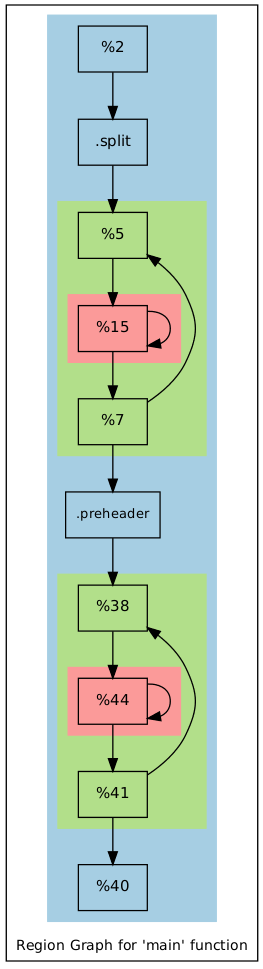
\includegraphics[width=\textwidth]{gfx/matmulRegions.png}
\end{figure}
\begin{sloppypar}
    \noindent
    For visualizing the regions of \autoref{lst:matmulcpp} a dot file is generated using the option \texttt{-view-regions-only}:
\end{sloppypar}
\begin{enumerate}
    \item Translate the C++ sourcecode of \autoref{lst:matmulcpp} into \llvmir (\autoref{lst:matmulll})\\
        \texttt{clang++ -S -emit-llvm matmul.cpp -o matmul.ll}
    \item Generate the regiontree\\
        \texttt{opt -view-regions-only matmul.ll}
\end{enumerate}
\subsection{Definition SCoP}\label{subsec:definitionScop}
\begin{comment}
    Copy\&pasted from polly/lib/Analysis/ScopDetection.cpp

    A static control part (Scop) is a subgraph of the control flow graph (CFG)
    that only has statically known control flow and can therefore be described
    within the polyhedral model.

    Every Scop fulfills these restrictions:
    * It is a single entry single exit region
    * Only affine linear bounds in the loops

    Every natural loop in a Scop must have a number of loop iterations that can
    be described as an affine linear function in surrounding loop iterators or
    parameters. (A parameter is a scalar that does not change its value during
    execution of the Scop).
    * Only comparisons of affine linear expressions in conditions
    * All loops and conditions perfectly nested

    The control flow needs to be structured such that it could be written using
    just 'for' and 'if' statements, without the need for any 'goto', 'break' or
    'continue'.

    * Side effect free functions call

    Function calls and intrinsics that do not have side effects (readnone)
    or memory intrinsics (memset, memcpy, memmove) are allowed.
\end{comment}

\begin{comment}
    The polyhedron model puts restrictions on the kind of programs that can be optimized.
    To be able to model a code region, it must have \textit{static control}.
    A code region with static control is called a static-control part or SCoP, for short. Loops should be for loops.
    A loop’s limits must depend only on structure parameters, numerical constants, and iteration variables of the enclosing loops.
    Structure parameters are integer variables whose values remain unchanged inside a SCoP.
    The statements in a SCoP may operate on linear data structures (typically arrays).
    Loop limits and array indices must be affine functions of the iteration variables and structure parameters. \cite{GanserIterativeSchedule}
\end{comment}

\begin{comment}
    May use quiet mathematical description of \cite{PolyhedralEmpiricalStudy}.
\end{comment}

A \scop is a specific region with further restrictions for being representable by the polyhedral model.\\
For being a valid \scop such a region has to have \enquote{static control flow}.
This includes that the region is a single entry single exit region, the loops within have to have only affine linear bounds, \eg the limits only depend on structure parameters\footnote{Structure parameter are integer variables whose values remain unchanged inside a \scop.}, numerical constants and iteration variables of enclosing loops. \cite{GanserIterativeSchedule, ScopDetection.cpp}
Further toplevel regions are excluded \draftnote{per default} from being a \scop not because of conceptional constraints but because Polly needs a safe space to put code for maintenance.
This means a \scop usually has maximum size if its parent is the toplevel region.\\
The visualization of the \scops of \autoref{lst:matmulcpp} is shown in \autoref{fig:exampleScop}.
\begin{figure}[!h]
    \centering
    \caption{The SCoPtree of \texttt{-O3} compiled \autoref{lst:matmulcpp}}
    \label{fig:exampleScop}
    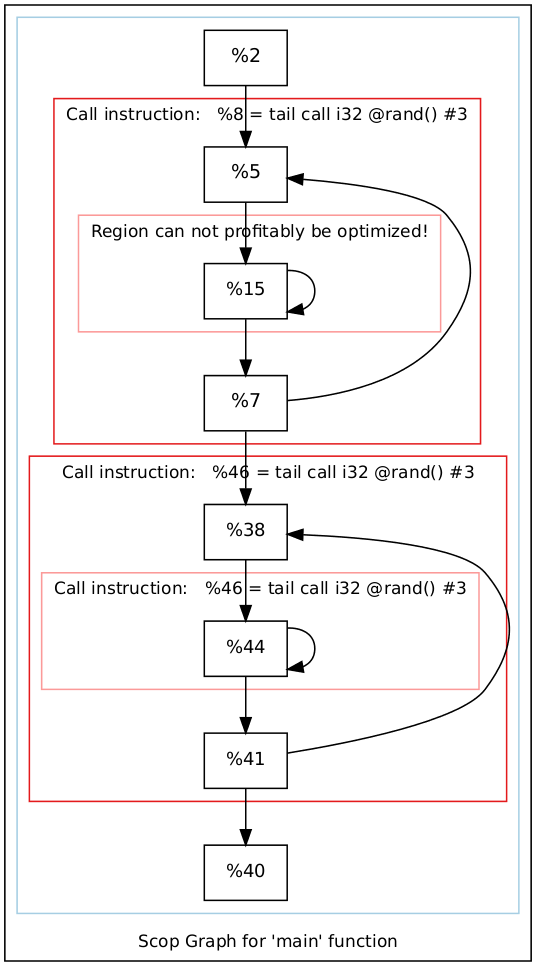
\includegraphics[height=\textheight]{gfx/matmulScops.png}
\end{figure}
The dot file is generated by the option \texttt{-view-scops-only}:
\begin{sloppypar}
    \begin{enumerate}
        \item Translate the C++ sourcecode of \autoref{lst:matmulcpp} into \llvmir (\autoref{lst:matmulllO3})\\
            \texttt{clang++ -S -emit-llvm \textbf{-O3} matmul.cpp -o matmulO3.ll}
        \item Prepare the \llvmir for Polly (\autoref{lst:matmulpreoptll})\\
            \texttt{opt -S -load LLVMPolly.so -polly-canonicalize matmulO3.ll > matmul.preopt.ll}
        \item Generate the \scop tree
            \texttt{opt -load LLVMPolly.so -disable-output -view-scops-only matmul.preopt.ll}
    \end{enumerate}
    On \autoref{fig:exampleScop} the regions of the \texttt{-O3} compiled \autoref{lst:matmulcpp} contain two \scops.
    These are the most inner regions described as \enquote{Region can not profitably be optimized!}.
    So these two can potentially applied loop optimizations on.
    In this case the option \texttt{-polly-process-unprofitable} has to be added to force Polly processing them although Polly classifies them as unprofitable.
\end{sloppypar}

\section{SCoPDetection}
To detect these \scops Polly searches in the first step for candidates using a top-down approach traversing the regiontree for canonical regions.
In the second step emanating from the candidates these are expanded until a \draftnote{marimal} region is found.
Afterwards \draftnote{in the modelling phase?} for every found candidate an optimized version of code is generated, which is surrounded by runtime checks for determing optimistically the provability of the correctness of the taken assumptions.
Following shows a list of assumptions possibly taken:
\begin{description}
    \item[Aliasing] Overlapping of the memory of variables \eg poiner onto some element of an array.
    \item[Inbounds] \draftnote{LLVM verwendet nur Pointer, keine Arrays. Eindimensionale Arrays rekonstruiert auf mehrdimensionale. => Abweichung Länge?}
    \item[Wrapping] Over- or underflow of short, integer,...
    \item[unsigned] \Eg overflow when using an unsigned integer as signed integer.
    \item[complexity] \draftnote{zu komplex?}
    \item[unprofitable] Overhead for generation of code extending the possible speedup.
    \item[errorBlock]
    \item[infiniteLoop]
    \item[invariantLoad]
    \item[delinearization]
\end{description}
\begin{comment}
    Copy\&pasted from ScopInfo.cpp

    STATISTIC(AssumptionsAliasing, "Number of aliasing assumptions taken.");
    STATISTIC(AssumptionsInbounds, "Number of inbounds assumptions taken.");
    STATISTIC(AssumptionsWrapping, "Number of wrapping assumptions taken.");
    STATISTIC(AssumptionsUnsigned, "Number of unsigned assumptions taken.");
    STATISTIC(AssumptionsComplexity, "Number of too complex SCoPs.");
    STATISTIC(AssumptionsUnprofitable, "Number of unprofitable SCoPs.");
    STATISTIC(AssumptionsErrorBlock, "Number of error block assumptions taken.");
    STATISTIC(AssumptionsInfiniteLoop, "Number of bounded loop assumptions taken.");
    STATISTIC(AssumptionsInvariantLoad,
              "Number of invariant loads assumptions taken.");
    STATISTIC(AssumptionsDelinearization,
              "Number of delinearization assumptions taken.");
\end{comment}
When the proof of the runtime check holds true, the optimized version of the code is continuing execution at that point.
Otherwise the execution jumps to the unoptimized version of the affected section.
\draftnote{
    \begin{itemize}
        \item Keine konservative Abschätzung
        \item Optimistische Abschätzung
            \begin{itemize}
                \item Annahme: Abhängigkeit existiert nicht
                \item Beweis zur Laufzeit (Laufzeitchecks)
                \item Test oft durch Kontradiktion => Z.T immer zurückspringen und keine Generierung von Code
                \item Falls nicht beweisbar, zurückspringen in unoptimierten Code
            \end{itemize}
    \end{itemize}
}
